\documentclass[11pt,a4paper]{article}

%% Preamble
\usepackage[utf8]{inputenc}
\usepackage{amsmath}
\usepackage{amsfonts}
\usepackage{amssymb}
\usepackage{url}
\usepackage{listings}
\usepackage{multicol}
\usepackage{hyperref}
\usepackage{graphicx}
\usepackage[colorinlistoftodos]{todonotes}

% For our todos we use the following colorcode:
% intern: only internal info, dont care
% urgent: all please have a look at it
% done: task solved, but would not mind a second person having a look at it

% the following todo commands take the arguments 
% \todo...[options]{author}{todomessage}
% options are the common options from the todonotes package and are an optional parameter
% for \todoin...[options]{author}{todomessage}{section}
% where todoin marks a whole section for refactoring or similar. 
\newcommand{\tododone}[3][noinline]{\todo[#1, author = #2, color=green!40]{\textit{#3}}}
\newcommand{\todointern}[3][noinline]{\todo[#1, author = #2, color=blue!40]{#3}}
\newcommand{\todourgent}[3][noinline]{\todo[#1, author = #2, color=red!40]{\textbf{#3}}}
\newcommand\todoindone[4][]{\todo[inline, author = #2, caption={#3}, #1, color=green!40]{
\begin{minipage}{\textwidth-4pt}\underline{#3}\\ \textit{#4}\end{minipage}}}
\newcommand\todoinintern[4][]{\todo[inline, author = #2, caption={#3}, #1, color=blue!40]{
\begin{minipage}{\textwidth-4pt}\underline{#3}\\  #4\end{minipage}}}
\newcommand\todoinurgent[4][]{\todo[inline, author = #2, caption={#3}, #1, color=red!40]{
\begin{minipage}{\textwidth-4pt}\underline{#3}\\ \textbf{#4}\end{minipage}}}

\lstset{%
  showstringspaces=false,
  breaklines=true,%
  frame=single,%
  language=C,%
  basicstyle=\small,%
  numbers=left,
  numberstyle=\tiny,
  basicstyle=\ttfamily\fontsize{10}{10}\selectfont,
  showstringspaces=false,
  showstringspaces=false}

\renewcommand{\arraystretch}{1.5}

\begin{document}


%%%%%%%%%%%%%%%%%%%%%%%%%%%%%%%%%%%%%%%%%%%%%%%%%%%%%%%%%%%%%%%%%%%%%%%%
% TITLE
%%%%%%%%%%%%%%%%%%%%%%%%%%%%%%%%%%%%%%%%%%%%%%%%%%%%%%%%%%%%%%%%%%%%%%%%

\title{Title-Needed: A framework for interactive computational fluid simulation and
visualization}
\author{Christie Alappat, Saumitra Joshi, Mohamed Khalil, Friedrich Menhorn,\\ Benjamin Rüth, Erik Wannerberg}

\maketitle

\tableofcontents

\listoftodos

%%%%%%%%%%%%%%%%%%%%%%%%%%%%%%%%%%%%%%%%%%%%%%%%%%%%%%%%%%%%%%%%%%%%%%%%
% INTRODUCTION
%%%%%%%%%%%%%%%%%%%%%%%%%%%%%%%%%%%%%%%%%%%%%%%%%%%%%%%%%%%%%%%%%%%%%%%%
\section{Introduction}
This is a framework for interactive simulation and visualization of
steered computational fluid and rigid body simulations.
It is based on pipelining concept further explained in Sec.\,\ref{sec:pipeline}
and a modular communication infrastructure.

This document gives an introduction to the basic concepts of the framework and
describes the requirements of it.

%%%%%%%%%%%%%%%%%%%%%%%%%%%%%%%%%%%%%%%%%%%%%%%%%%%%%%%%%%%%%%%%%%%%%%%%
% Requirements \& Compilation
%%%%%%%%%%%%%%%%%%%%%%%%%%%%%%%%%%%%%%%%%%%%%%%%%%%%%%%%%%%%%%%%%%%%%%%%
\section{Requirements \& Compilation}

The project was developed to be compiled and executed on Ubuntu 12.04 LTS
\footnote{\url{http://www.ubuntu.com/download/desktop}}.

After downloading and installing the system, several packages are required.
Those can be installed using \textit{apt-get} from the command line.

\begin{lstlisting}[language=sh]
$ apt-get install libsdl-image1.2-dev libsdl1.2-dev libv4l-dev g++
$ apt-get install git
$ apt-get install libcv-dev libcvaux-dev libhighgui-dev libcv2.4 libhighgui2.4 libcvaux2.4 opencv-doc
$ apt-get install cmake freeglut3-dev pkg-config build-essential libxmu-dev libxi-dev libusb-1.0-0-dev doxygen graphviz mono-complete git-core
$ apt-get install libopenblas-dev liblapack-dev libarpack2-dev
$ apt-get install valgrind
\end{lstlisting}

If you have an NVIDIA-GPU and want to use it, you should install CUDA as well. To do this, 
first install the latest proprietary driver via the "Additional Drivers" Tool in Ubuntu.
Then, follow the instructions of this \href{www.r-tutor.com/gpu-computing/cuda-installation/cuda7.0-ubuntu}{How-To} 
(but use the stuff for ubuntu 14.10 - there's no .deb-package for Ubuntu 15.04 yet,
but this one works just fine)

For eclipse development environment, additionally install java jre
\begin{lstlisting}[language=sh]
$ apt-get install default-jre
\end{lstlisting}

After installation of the required packages, the code can be compiled with

\begin{lstlisting}[language=sh]
$ make
\end{lstlisting}

In case that you get any compilation errors, please send your advisors an
email. The program will be located in the build folder and can be run by

\begin{lstlisting}[language=sh]
$ ./build/fa_2014_release
\end{lstlisting}

%%%%%%%%%%%%%%%%%%%%%%%%%%%%%%%%%%%%%%%%%%%%%%%%%%%%%%%%%%%%%%%%%%%%%%%%
% Code Framework
%%%%%%%%%%%%%%%%%%%%%%%%%%%%%%%%%%%%%%%%%%%%%%%%%%%%%%%%%%%%%%%%%%%%%%%%
\section{Code Framework}


%%%%%%%%%%%%%%%%%%%%%%%%%%%%%%%%%%%%%%%%%%%%%%%%%%%%%%%%%%%%%%%%%%%%%%%%
% Classes
%%%%%%%%%%%%%%%%%%%%%%%%%%%%%%%%%%%%%%%%%%%%%%%%%%%%%%%%%%%%%%%%%%%%%%%%

\subsection{Classes}
There are a bunch of existing classes which should be used by everyone to setup
the interfaces among the groups.
The following table gives an overview and short description of each class.

\noindent
\begin{tabular}{|l|l|}
	\hline
	CDataArray2D.hpp				&
		Data storage for 2D arrays							\\
	\hline
	CDataDrawingInformation.hpp		&
		Data storage for interactive drawing information	\\
	\hline
	CGlTexture.hpp					&
		Abstraction for OpenGL Textures						\\
	\hline
	CParameters.hpp					&
		Program and simulation parameters					\\
	\hline
	CPipelinePacket.hpp				&
		Pipeline packet capable of being forwarded via the pipeline	\\
	\hline
	CPipelineStage.hpp				&
		Pipeline stage providing interfaces for pipelining	\\
	\hline
	CSDLInterface.hpp				&
		SDL Interface for visualization and interactivity	\\
	\hline
	CStage\_ImageInput.hpp			&
		Pipeline stage for image input (single image from file)	\\
	\hline
	CStage\_ImageProcessing.hpp		&
		Pipeline stage for image processing filter			\\
	\hline
	CStage\_VideoInput.hpp			&
		Pipeline stage for video input, e.g.\,from webcam	\\
	\hline
	CStage\_VideoOutput.hpp			&
		Pipeline stage for video output				\\			
	\hline
	main.cpp						&
		main entry to setup pipelined scenarios		\\
	\hline
\end{tabular}


%%%%%%%%%%%%%%%%%%%%%%%%%%%%%%%%%%%%%%%%%%%%%%%%%%%%%%%%%%%%%%%%%%%%%%%%
% Pipeline
%%%%%%%%%%%%%%%%%%%%%%%%%%%%%%%%%%%%%%%%%%%%%%%%%%%%%%%%%%%%%%%%%%%%%%%%
\subsection{Pipeline}
\label{sec:pipeline}

The idea of a pipelining model is creating independent execution parts with
particular input-output specifications.
E.g.\,a webcam only provides images which are forwarded to the image filter.
After processing of the image filter, this information is further forwarded to
the simulation (not yet implemented) and then to the output for visualization.

All those pipeline stages are independent and thus can be independently
processed - e.g. Image filter and simulation computations in parallel.

%%%%%%%%%%%%%%%%%%%%%%%%%%%%%%%%%%%%%%%%%%%%%%%%%%%%%%%%%%%%%%%%%%%%%%%%
% Pipeline stage
%
\subsubsection{Pipeline stage}

We continue with an example given by the image processing filter
\textit{CStage\_ImageProcessing.hpp}.
For well-known interfaces, each new pipeline stage has to inherit the class
CPipelineStage:

\begin{lstlisting}
class CStage_ImageProcessing	:	public
	CPipelineStage
...
\end{lstlisting}

\noindent
For processing of the images, paramters are required to know which
computations to do, at least a single input storage is required as well as an
output storage to forward processes images to other classes:

\begin{lstlisting}
...
/**
 * global parameters
 */
CParameters &cParameters;

/**
 * input image
 */
CDataArray2D<unsigned char,3> input_cDataArray2D;

/**
 * processed image
 */
CDataArray2D<unsigned char,3> output_cDataArray2D;
...
\end{lstlisting}

\noindent
Since the parameters are shared with the other classes, they are
setup in the constructor:

\begin{lstlisting}
public:
/**
 * constructor
 */
CStage_ImageProcessing(CParameters &i_cParameters):
CPipelineStage("ImageProcessing"),
cParameters(i_cParameters)
{
}
\end{lstlisting}

\noindent
In case of an input sent via the pipeline of another stage such as the video
input, the method \textit{pipeline\_process\_input} is executed and has to be
implemented. This interface is particularly requested by the class
\textit{CPipelineStage}.

\begin{lstlisting}
void pipeline_process_input(
	CPipelinePacket &i_cPipelinePacket
)
{
...
\end{lstlisting}

\noindent
Since not all possible data types can be probably processed, we have to check
for compatible input packages and unpack the data to make it available with our
accessor class:
\begin{lstlisting}
// we are currently only able to process "unsigned char,3" data arrays.
if (i_cPipelinePacket.type_info_name != typeid(CDataArray2D<unsigned char,3>).name())
{
	std::cerr << "ERROR: Video Output is only able to process (char,3) arrays" << std::endl;
	exit(-1);
}

// unpack data
CDataArray2D<unsigned char,3> *input = i_cPipelinePacket.getPayload<CDataArray2D<unsigned char,3> >();
\end{lstlisting}

\noindent
After unpacking the data and processing the data with more details available in
the source code file itself, the output data array is pushed to the pipeline and
thus forwarded to the next pipeline stages:
\begin{lstlisting}
CPipelineStage::pipeline_push((CPipelinePacket&)output_cDataArray2D);
\end{lstlisting}

%%%%%%%%%%%%%%%%%%%%%%%%%%%%%%%%%%%%%%%%%%%%%%%%%%%%%%%%%%%%%%%%%%%%%%%%
% Pipeline setup
%
\subsubsection{Pipeline setup}
After programming several stages, their input and output has to be
connected after instantiation.
E.g.\,let us assume that we like to have an static input image with an image
filter and the possibility to draw into the image, this would lead to the
following pipeline:

\begin{lstlisting}
// static image input
CStage_ImageInput cStage_ImageInput(cParameters);
// video output
CStage_VideoOutput cStage_VideoOutput(cParameters);

// PIPELINE CONNECTIONS
// forward image to video output
cStage_ImageInput.connectOutput(cStage_VideoOutput);
// forward mouse movements to image input
cStage_VideoOutput.connectOutput(cStage_ImageInput);


// initial push of static image
cStage_ImageInput.pipeline_push();

// main loop
while (!cParameters.exit)
{
	// trigger image input to do something
	cStage_VideoOutput.main_loop_callback();
}
\end{lstlisting}

\noindent
For our pipeline concept, only the outputs have to be connected.
The initial push for the image input is required to initially forward the static
image to the video output.

The main loop is required to e.g.\,check for user input, to draw updates for the
visualization and to run a simulation timestep.


\subsection{Interaction}
Several keystrokes currently exist updating some parameters in the class
\textit{CParameters}.
Note that all pipeline stages get a reference to this class during
initialization.

Since the Video output is closely connected to the input system, all
input keystrokes which are not directly processed are forwarded to the method
key\_down of the parameter class:

\begin{lstlisting}
/**
 * return bool if processed
 */
bool key_down(char i_key)
{
	switch(i_key)
	{
	case SDLK_j:
		stage_imageprocessing_filter_id--;
		std::cout << "Using filter id " << stage_imageprocessing_filter_id << std::endl;
		return true;

	case SDLK_k:
		stage_imageprocessing_filter_id++;
		std::cout << "Using filter id " << stage_imageprocessing_filter_id << std::endl;
		return true;
\end{lstlisting}

\noindent
This allows the modification of the parameters during the programs runtime.
So far the following keystrokes are defined:

\noindent
\begin{tabular}{|c|l|}
	\hline
	\multicolumn{2}{|l|}{\textbf{General}}	\\
	\hline
	q & quit program	\\
	\hline
	\hline

	\multicolumn{2}{|l|}{\textbf{1: image Processing}}	\\
	\hline
	j,k & decrease / increase filter id\\
	\hline
	g,t & decrease/increase threshold value\\
	\hline
\end{tabular}


\subsection{Program start}

Several program parameters currently exist and are also processed in
CParameters:

\noindent
\begin{tabular}{|c|l|}
	\hline
	\multicolumn{2}{|l|}{\textbf{General}}	\\
	\hline
	p	& pipeline id to use (see main.cpp)	\\
	\hline
	v	& verbosity level	\\
	\hline
	\hline

	\multicolumn{2}{|l|}{\textbf{0: image/videoinput}}	\\
	\hline
	d	& video device string to use\\
	\hline
	w	& request this width for video input\\
	\hline
	h	& request this height for video input\\
	\hline
	i	& path to input image to use\\
	\hline
	\hline

	\multicolumn{2}{|l|}{\textbf{3: fluid simulation LBM}}	\\
	\hline
	v	& switch between flag field and velocity output	\\
	\hline
	\hline
	
	\multicolumn{2}{|l|}{\textbf{4: parallelization}}	\\
	\hline
	n	& number of threads to use\\
	\hline
	\hline

\end{tabular}
\newpage

%%%%%%%%%%%%%%%%%%%%%%%%%%%%%%%%%%%%%%%%%%%%%%%%%%%%%%%%%%%%%%%%%%%%%%%%
% The Different Teams
%%%%%%%%%%%%%%%%%%%%%%%%%%%%%%%%%%%%%%%%%%%%%%%%%%%%%%%%%%%%%%%%%%%%%%%%
\section{Project Management}
\tododone[inline]{Mohamed}{\textbf{Project Management}}
\tododone[inline]{Benni}{did proofreading}
This section will give an insight into the recommended management strategy to be used for this kind of project and give an overview over the necessary managerial tools suggested for similar projects in the future.
\todointern[inline]{Benni}{move this to challenges and pitfalls section?}
We will also show up the challenges that will probably show up along the way as well as strategies for avoiding pitfalls.

\subsection{Agile Management}
%\textit{Here a brief introduction on agile management will be given with minimal theoretical details (since we always minimze in agile)}
Agile management is a management strategy which is commonly used in software development projects. It is very flexible with respect to developers changing decisions and customers updating their needs. The principle of this management scheme is to divide the full project into smaller chunks, referred to as sprints. Each chunk involves finishing a fully working part of the project. For example, in our project theme, a possible set of sprints could have been:
\begin{enumerate}
  \item{Setting up all interfaces with dummy data to complete the pipeline}
  \item{Replace the dummy data with real data via implementing the necessary models or wrapping the available libararies}
  \item{Adding different levels to the game via image processing and implementing a more complex rigid body representation}
  \item{Allowing the user to draw the levels}
  \item{etc...}
\end{enumerate}
It can be observed that at the end of each sprint the entire code is running, integrated and producing some kind of output (despite its 	plausibility). During each sprint the output keeps developing and iteratively approaches its final shape. In addition the developers do not walk into the trap of being involved in their part while they are hoping that at some distant point in future, they will merge their code with the other teams' and everything will run smoothly. Moreover, this method allows for continuous unit-testing (explained in \autoref{unit_testing}) and early error correction.
One favourable aspect about agile management also is the resulting flexibility in human resources management through relocation and collocation. Relocation is the shuffling of one person's assignment from one team to another after completing the tasks in the respective team or if the team is no more in need of all the manpower. Collocation, on the other hand, is the distribution of one person among more than one team of developers, which is specially encouraged for people handling data interfaces between different teams.

\subsection{Useful Organizational Tools}
In this section, the light will be shed upon the methodology adopted by our group for deciding the project's theme and the concept of scrumming will be exposed. In addition, other facilitation tools will be presented.

\subsubsection{Project's Selection For Dummies}
Project selection is the first step in implementing it. With the flow of ideas and a wide spectrum of imagination among the developers on their first gatherings, they are suddenly confronted with a huge range of project ideas, that for the first glance seem appealing. However, project selection is more than just the vibrance of the idea. The following section will detail some tips on guiding the project selection.

\begin{itemize}
  \item \textbf{Brainstorming}: The first step in choosing a project topic is to set the sky as the limit for people to pour out their ideas all together into one pool, and most importantly, out-loud, allowing people to generate more ideas and develop one another's. An important aspect to be aware of is not to let this stage take a very long time, since time at Ferienakademie is somehow restricted. Also, it is be very helpful to find common grounds between different ideas as soon as possible. For example, "all the proposed ideas will require a Kinect input interface" or "regardless the topic we eventually select, we will need an fluid-structure-interaction framework". Reaching such conclusions early initiates the project in concurrency with finalizing/elaborating the ideas.
  
  \item \textbf{Selection Matrix}: It is very crucial and helpful to decide upon some criteria to evaluate the quality of the idea. On first sight one will assume that all ideas are creative and extravagant -- and it is of course desirable to have such an output -- but their charm might dim after being inspected subjectively with respect to criteria such as:
  \begin{itemize}
    \item \textit{Usability}: How easy can the end-user play this game or use this program? Will he/she need an intensive documentation or a direct supervised training or instructions to start using the game correctly?
    \item \textit{Realizability}: How good is the idea realizable? Can we reach a very simple first state with low effort?
    \item \textit{Extensibility}: How far can we go beyond the first milestone? Can we add more features to the project to make it more challenging and interesting?
    \item \textit{Audience-interest}: How attractive it is for audience to watch the game? For example, chess is a big fail even if you like it!
    \item \textit{Developers-interest}: Are we eager to put all our effort for around 10-days on that project?

  \end{itemize}
For our project, having a matrix (with projects' proposals on one edge and criteria on the other), the developers simply agreed a grade for each criterion for every idea and points we counted.
Automatically, some ideas dropped out and it was obvious towards which idea(s) the decision is heading. In case more than one project got close high ranks, their ideas might be re-discussed and re-evaluated for the final decision. If one cannot come up with a decision a hike often helps.
\end{itemize}


\subsubsection{Scrumming}
%\textit{An idea about scrumming, what are they used for, the sort of updates discussed through them, etc.}
The term scrumming in agile management is inspired by the first move in an American football game, where all the players from each team initially start at the centerline and then in a glance spread all over the field - that move is the \emph{scrum}. The idealisation of such a concept in software development is such that the developers meet frequently (usually weekly or biweekly, at Ferienakademie of course more frequently) to discuss the following three points:
\begin{itemize}
  \item{What has been achieved/completed since the last scrum?}
  \item{What is the prospective task until the next scrum?}
  \item{Have any challenges popped up that require help from other developers?}
\end{itemize}
The main idea of scrumming is to keep all developers and the manger(s) aware of the current status of each separate area in the project and of what each team has achieved so far. 
Scrums are neither for feedback on the project or the developers nor for brainstorming. 
In our case, the scrum was held almost every morning, and if needed, it was rescheduled to a different time during the day, but generally we had a daily scrum. Our team consisted of about 20 developers and having all those in one meeting was thought to be hectic. Hence, for every team, a representative was chosen to attend the scrum and update on behalf of his team. Nevertheless, involving the entire team in the meeting doesn't sound like a bad idea since it could provide an even more detailed insight about the progress of each team (versus the general statement about the progress given by the representative). Additionally this encourages a more direct communication channel between members from different teams dealing with common issues (such as interfaces). \todo{lesson learned? I think this only makes sense after the respective sections.} In our project, I guess, it would have helped to have the developers of the LBM team listen directly in scrums from the RB team and vice versa.

\subsubsection{Code Handling Facilitators}
One of the duties of the project management is to ensure that code is being handled smoothly within the team. Our team has found the following tools pretty beneficial while working on the project.

\begin{itemize}
  \item \textbf{Git}\footnote{An alternative code management tool could be SVN}: for organized code sharing without conflicts, repository updating with current work, experimenting safely with developers' ideas on separate branches, managing conflicts between coders' work, etc. (for managing merge conflicts we suggest \href{meld}{http://meldmerge.org/})
  \item \textbf{CMake}: for a more neat and modular compilation of the whole project from one parent directory
  \item \textbf{Valgrind}: for debugging the code and hunting malicious code lines that result in segmentation faults and other nasty bugs
  \item \textbf{Unit-testing}\footnote{Boost provides a good unit testing tool for C++}: testing each block of code or every interface separately with hardcoded example data to make sure it is bug free and interacting safely with given input and providing sensible output before handling it to the other teams up- and downstream the pipeline\label{unit_testing}
  \item \textbf{Code References}: since we were in an internet-deserted area, having an offline chest of language references and library documentation is worth a fortune. Useful documentations are library's supplier-provided documentation, c++ reference and an offline repository of stackoverflow (and might as well for other libraries used if no PDF documentation was found\todointern{Benni}{what? I don't understand the sentence...})
\end{itemize}

\subsection{Challenges and Obstacles}
\todourgent[inline]{Benni}{Move this part in a final summary chapter? Summary and lessons learned}
Challenges are not bugs, they are features, and one should be indeed aware of their existence and do his/her best to avoid them or at worst be ready to handle them if they can't be detoured \todointern{Benni}{do your best to avoid challenges! Surprising attitude for a BGCE student :P}. Some challenges that we experienced through our project are listed below.

\begin{itemize}
  \item \textbf{Time constraint}: We had many hikes, plus there were a couple of social gatherings and events such as the tournaments and the cultural evening. This boiled down two weeks of work dedicated to the project to much less time. This aspect needs to be taken into account when setting the milestones for the project.
  \item \textbf{Defining the project's topic}: Due to the multi-disciplinary background of the participants as well as various interests, the brainstorming session turns out really vibrant between different ideas. Attention should be drawn to common grounds and the manager(s) should at some point occlude the ongoing flow of ideas to agree onto something.
  \item \textbf{Defining the milestones (be really to \todo{?} agile)}: One of the challenges faced in our projects was phrasing the first milestone deliverables thorough-enough. The first milestone deliverable should not have been just about "Create a game with the simplest fluid-structure interaction and only taking input from Kinect". Such a statement comprised too much of details to work on such as the level of details of rigid bodies capabilities. In addition, it required a comprehensive data handling system between different pipeline stages, which implied that each team should necessarily implement fully-working functionality in order to test the pipeline integrity (imagine how long could this have taken !!).
  A more efficient/agile approach would have been to set the first milestone deliverable to be "building and closing the pipeline with dummy data". This would have crossed out a milestone from the list and given all the teams an insight about into the interaction with the preceding and proceeding pipeline stages.
  \item \textbf{Testing the code}: With around 20 developers, each one implementing a chunk, the code is very vulnerable to get broken by some mathematical fault in a function or a segmentation-fault in one group's code. This could be avoided -- up to some extend -- by unit-testing. Unit-testing is hard-coding an example in order to test the implemented methods and ensure that they are giving the expected response. Although unit-testing requires a considerable additional workload, it, on the other hand, saves the programmers a lot of debugging time in case something goes wrong. This was extremely crucial in the interface between rigid bodies and LBM due to the massive amount of communication between the two codes.
  \item \textbf{Waterfalling}: Waterfall differs from agile management in that it treats the project as a one whole and the tangible output is only delivered at the end. This could be inefficient in projects like ours since waiting till the end since the developers might get demotivated as time passes without tangible output\todo{?}. Also, the project becomes more rigid to adding or modifying milestone deliverables for later stages. The risk of waterfalling is usually high when the first milestone is not clearly bounded and be made aware to the developers. The risk evolves that they end up indulging into coding and extending functionality of their blocks, while delaying integration of their respective parts with the others on the pipeline.
  \item \textbf{Speaking German}: Although the course's official language is English, nevertheless, one can't hold a group of 90\% of Germans to speak their mother language. In such an environment, non-formal meetings between developers (meaning small talks during coffee breaks, discussion over lunch, casual chats, etc.) encourage ideas flow and facilitate problem solving among developers as well as helps management to be updated with deeper details of the project's status. It is rather recommended that the managers' language skills in later courses is good enough to engage and comprehend such situations easily and not just rely on the English scrum meeting for udpates.
\end{itemize}

\todoinintern{}{additional stuff for lessons learned}{ 
\begin{itemize}
\item Managers should not distribute among groups, but manage the team and mistrust everybody. 
\item A group dedicated to game logic (became part of rigid bodies job...) and level design would have been good. 
\item Visu people used OpenGL (very rigid, only runs on some computers, BUT powerful), SDL was the intended language (default in sceleton). Maybe presentation on SDL would have been good? Are there also other possible presentation topics, we missed during ferienakademie?
\end{itemize}
}



\section{Input Devices}
\tododone[inline]{Benni}{Erik responsible for section \textbf{Input Devices}}
\todointern[inline]{Erik}{If someone proofreads it'd be nice, I might ask Steffen}
\todointern[inline]{Mohamed}{did proofreading}

To be able to control our game interactively, we need to have some means of providing input during runtime, and this is where the Input Devices come into play. Two different kinds of devices were used in the final game; first, to control the boats, paddling gestures were interpreted by a Microsoft Kinect\footnote{For those who do not know, the \emph{Kinect} is a motion-tracking device developed by Microsoft initially for their gaming console Xbox 360, which can track bodies by analysing a depth field of the view in front of it, provided by an IR camera. For a more in-depth description, see for example \url{http://www.i-programmer.info/babbages-bag/2003-kinect-the-technology-.html}.}, and, second, keyboard inputs were used, for example, to quit the program or change the views for debugging purposes. Additionally, a mode without Kinect was available, which allowed two players to control the boats with the keyboard. In this section, we will look closer at how we used them and how to interface with such devices, and breifly mention how it can work for a Nintendo Wii controller (\emph{Wiimote}), which was initially considered for usage but rejected during the project.

\subsection{Usage}
The usage of the Kinect in the game is (at least in theory) very simple.
\begin{itemize}
\item To use the Kinect, one needs to provide the command line argument \texttt{-dKinect} to select the Kinect as the steering device.
\item After the game has started, the Kinect software has to recognize a person to start tracking him/her. To be recognized, one stands in front of the Kinect (optimal distance 2.5m) and holds the \emph{Calibration Pose}, which in our case is standing straight with the arms upwards in a "U"-shape, such that the whole body forms the greek letter capital \emph{Psi} $\Psi$.
\item After one person has done so, a message on the screen tells the user that "\emph{Player 1 recognized}". However, since our game requires two people, the same procedure has to be repeated for a second person, who will be "Player 2" in the game.
\item After both people have been recognized, the picture changes to one where the two boats are visible, and the game starts.
\item The players then try to paddle their way from the start (typically on the left side of the level's screen) to the goal (typically on the right side) and to get there before the other player.
\item And how does this paddling work? The player makes motions similar to that while paddling in a canoe: with both hands, one above the other, move an invisible paddle from the front to the back, again and again, to one side of the body. This creates a forward force with each paddle stroke. 
\item Of course, one also has to steer: depending on which side of the body the player strokes, the force also starts turning the boat either left or right; a stroke on the left side of the body makes the boat rotate clockwise, turning the boat to the right, and vice versa for turning in the opposite direction.
\item Just like in reality, the further out one strokes\footnote{Here interpreted by the angle of the imaginary paddle between the player's hands to the line that goes through the person's shoulders. That means, if you stand upright, and paddle with your hands almost parallel to the ground, you will turn a lot; if you hold one straight above the other, you will turn much less.}, the more the boat will turn.
\item Also, the faster you move your paddle, the more force you will provide to the boat, and you will go faster!
\end{itemize}
\todointern[inline]{Mohamed}{Shall we add that this calibration was proposed by us, ut others might come up with different scenarios to interpret the motion.. I mean that's not a Kinect default calibration}

The game also provides ways of interacting by keyboard:
\begin{itemize}
\item If you are unlucky enough not to be able to use a Kinect, don't worry, you can still play "Grand Theft Boat - Sarntal" using the keyboard as the steering device! If you provide the command-line input \texttt{-dKeyboard} (or indeed nothing at all, since this is the default case), Player 1 can steer his or her boat using the keyboard keys \texttt{a} and \texttt{s}, which will simulate a left-side and right-side paddle stroke, respectively. Player two will compete by using the keys \texttt{n} and \texttt{m}.
\item Other keyboard commands include \texttt{q} for quitting the game, keys \texttt{1-9} for different camera options, and \texttt{v} for toggling debug output related to the velocity field.
\end{itemize}



\subsection{Installation}
In order to install the libraries that provide Kinect\footnote{Namely OpenNI \cite{OpenNI}, a 3D sensor framework for bridging different devices to a uniform API, the NITE algorithms, which are middleware that provide body recognition in the same framework, and SensorKinect \cite{SensorKinect}, an open source driver for the Kinect that plugs into OpenNI.} and Wii integration\footnote{WiiC \cite{WiiC}, an open source, lightweight library that can handle different Wii controllers via bluetooth, which thus also depends on bluetooth hardware and drivers, and BlueZ in particular.}, take a look at the folders \texttt{fa/sources-for-kinect} and \texttt{fa/sources-for-wii}. Please read the corresponding README files inside and do what it says. The keyboard input is handled by the \emph{Simple DeviceMedia Library} (SDL), which also handles graphical output, which requires the installation of \texttt{libsdl} included in the skeleton described above. The native Xbox Kinect also requires an adapter to allow it to be connected to a computer's USB port.

\subsection{Implementation}
The device inputs are handled in several different places in the code; firstly, in the first pipeline stage in the class \texttt{CStage_DeviceInput}. Here, if Kinect input was specified, OpenNI-implementing functions in \texttt{DeviceHandler.hpp} and \texttt{ControlPaddle.hpp} are called, and if keyboard input is specified, SDL functionality in \texttt{ControlKey.hpp} is called. In both of these places, the input is converted to a force and a torque, which are sent as a \texttt{CPipelinePacket} subclass to be handled in the Rigid Body part of the code.

Keyboard commands are also handled in the video output pipeline stage \texttt{CStage_VideoOutput}, where it is used to control the camera, and if not matched, passed on to the \texttt{CParameters} class for checking against quitting parameters or similar.


%\begin{itemize}
%\item we only used kinect
%\item shortly describe kinect input gestures and necessary steps to get the rowing movement detected and correctly resolved
%\item what do we do with the input? Forward it to rigid bodies!
%\end{itemize}


\section{Image Processing}
\label{sec: imageProcessing}
\tododone[inline]{Saumi}{Section done.}

One of Grand Theft Boat's USPs is the freedom for players to fully customize their level maps. Players can design complex maps replete with shorelines, connected water bodies, and floating spherical obstacles of varying radii. All this can be done using a simple computer graphics software like Gimp (Linux), MS Paint (Windows) and Paintbrush (Mac). 

\begin{figure}
\centering
  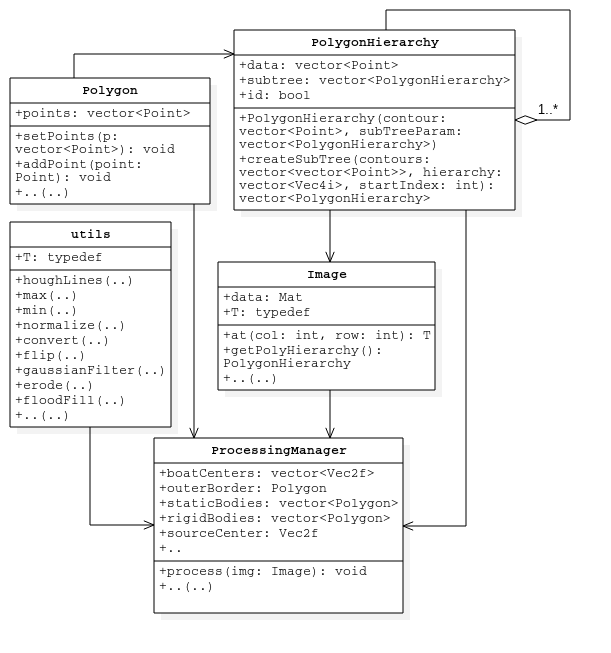
\includegraphics[scale=0.6]{img/ImageProcessing/UML_ImgProc_PNG.png}
\caption{UML diagram for the image processing code\label{fig:UMLImgProc}}
\end{figure}

In order to extract information about the terrain and participating bodies, the team relied on processing the input image through extensive use of the OpenCV library. This chapter describes the workflow involved in this stage. The broad structure of the image processing code is shown in Figure \ref{fig:UMLImgProc}.

The other parts of the code interact with the Image Processing section through an instance of \verb|ProcessingManager|. This class takes an image from the player, processes it to extract and store information about different terrain objects, and provides functions to return this information when required by other sections.

\subsection{Level Terrain Specification}

\begin{figure}
\centering
  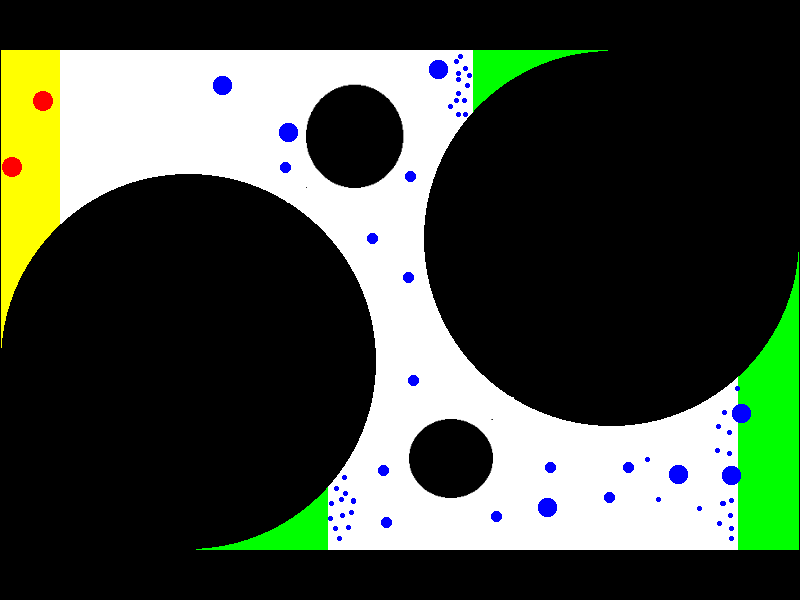
\includegraphics[scale=0.4]{img/ImageProcessing/LevelImages/img_0.png}
\caption{A typical player input for specifying the desired layout of the level\label{fig:LevelInput}}
\end{figure}

Figure \ref{fig:LevelInput} shows an example of a player's level specification.
\begin{itemize}
	\item Regions colored black represent land. This part of the domain is not a part of the solution field. The part of the black that borders the white region is treated as a rigid boundary.
	\item White-colored regions represent the water body. This space is the actual solution domain of the fluid.
	\item Green patches represent sources of momentum for the fluid.
	\item Yellow patches are sinks for the fluid. (See the section on LBM for the mathematical meaning of sources and sinks.
	\item Red spheres indicate the initial position of the player boats.
	\item Blue spheres create obstacles as rigid bodies.
\end{itemize}


\subsection{Pre-Processing}

Many a time, the image supplied by the player may need to be pre-processed for improving boundaries between terrain types. Once given as input to the \verb|ProcessingManager|, the input image undergoes the following sequence of filters:

\begin{enumerate}
	\item \textit{Flip image}: 
	
	\verb|img = img::flip(img, true, false);|
	
	Flipping the image along the y-axis is necessary because the coordinate system of a standard image has its origin on the top-left corner, while standard fluid codes begin indexing from the bottom-left corner.

	\item \textit{Gaussian filter and opening}

	\verb|blurred = img::gaussianFilter(img, 7, 2);|

	\verb|opened = img::opening(blurred, structuringElement, 2);|
	
	The gaussian filter and opening helps eliminates fuzzy borders of adjacent colors, making them sharper. See Figure \ref{LevelImages}(a).

	\item \textit{Thresholding}

	\verb|thresholded = applyThresholding(opened);|
	
	Thresholding applies yes-no filters on the image based on the colors of different domain types. This provides the \verb|ProcessingManager| with a boolean (black-white) image for each domain type, which is then used to extract domain information.

\end{enumerate}


\subsection{Information Extraction}

\begin{figure}
\begin{tabular}{cc}
  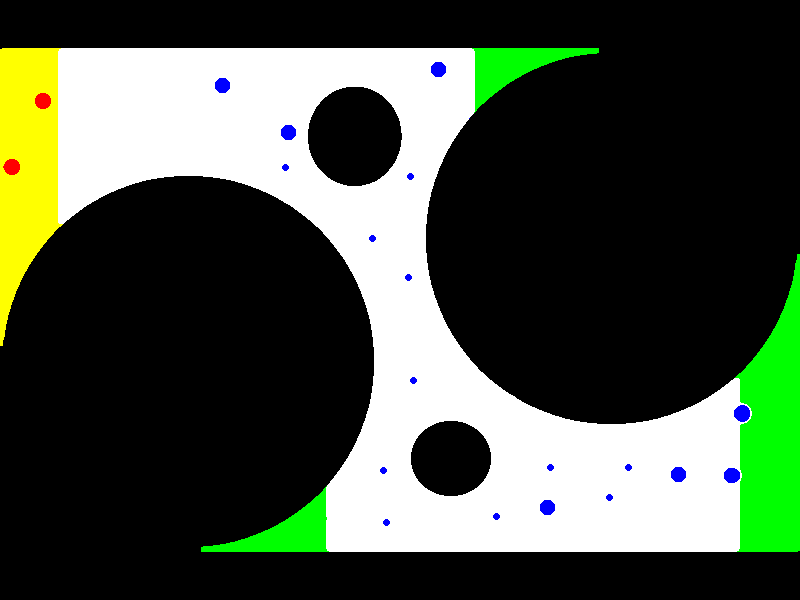
\includegraphics[width=65mm]{img/ImageProcessing/LevelImages/img_3.png} & 
\includegraphics[width=65mm]{img/ImageProcessing/LevelImages/img_5.png} \\
(a) & (b) \\[6pt]
  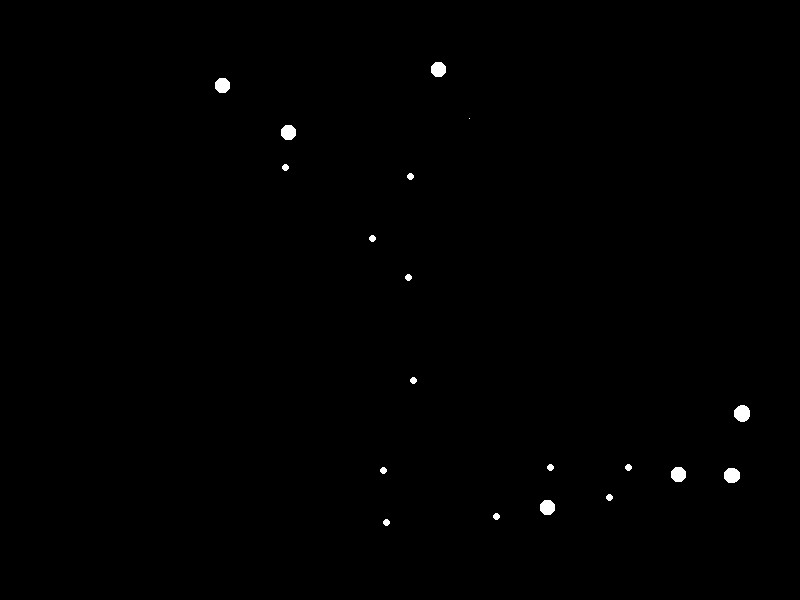
\includegraphics[width=65mm]{img/ImageProcessing/LevelImages/img_10.png} & 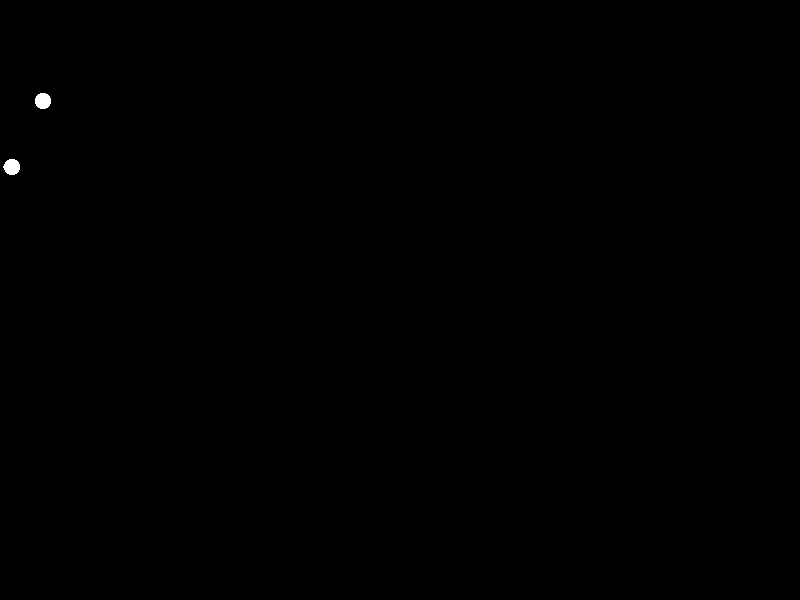
\includegraphics[width=65mm]{img/ImageProcessing/LevelImages/img_12.png} \\
(c) & (d) \\[6pt]
\end{tabular}
\caption{Various stages of processing the image. (a) After pre-processing, (b) image for \protect\lstinline|outerBorder| and \protect\lstinline|staticBodies|, (c) image for \protect\lstinline|rigidBodies|, and (d) image for \protect\lstinline|boatCenters|.\label{LevelImages}}
\end{figure}

The pre-processing brings the image in a state where information about the terrain can be easily extracted from it. Various information extraction techniques are applied to this processed image to obtain terrain information relevant to the simulation.

\begin{itemize}
	\item \textit{Sources}: Detected by a simple color comparison.
	\item \textit{Boats}: Boat pixels detected by color comparison. Their centers are located by a k-means analysis for 2 buckets. See Figure \ref{LevelImages}(d)
	\item \textit{Rigid Bodies}: The first step in the detection of the rigid body obstacles is the isolation of the obstacles as a binary "obstacle or not-obstacle" image. This is done by a series of boolean operations (provided in class \lstinline|utils|). This image is then supplied to the class \lstinline|PolygonHierarchy|.

The class \lstinline|PolygonHierarchy| is a recursive class holding two parameters: 
	\begin{itemize}
		\item \lstinline|data|: a set of points forming a closed polygon.
		\item \lstinline|subtree|: a vector of \lstinline|PolygonHierarchy|.
	\end{itemize}
The level of a \lstinline|PolygonHierarchy| indicates how many outer polygons enclose the polygons at that level. Note that the zeroeth-level \lstinline|data| is empty.

This \lstinline|PolygonHierarchy| is applied on Figure \ref{LevelImages}(c), and the first-level polygons give the rigid body obstacles.

	\item \textit{Fluid Domain}: The fluid domain is extracted in a similar manner by choosing the first-level polygon for Figure \ref{LevelImages}(b).

	\item \textit{Static Bodies}: The static bodies are detected by choosing the second-level polygons for Figure \ref{LevelImages}(b).

\end{itemize}


The Image-processing-group also performs the task of writing the flag field for the LBM-group. The flag field is scaled to the desire screen pixel resolution. All the information extracted so far is stored in the \verb|ProcessingManager| and passed on to the Rigid-body-group (for obstacles, shorelines and boats) and the LBM-group (for the flag fields).


\section{Lattice Boltzmann simulation}

let your thoughts just flow

\section{Rigid Body Simulation}
\tododone[inline]{Benni}{responsible for section \textbf{RB}: Friedrich -- DONE}
\todourgent[inline]{Benni}{did some proofreading and minor corrections}

The goal of this project was to develop a game which is based on a real time physics simulation of fluid flow, rigid bodies and their interaction. The main task of the rigid body group was hence the collision detection and collision handling for the different objects as well as developing the interface to the fluid group, which gives us the necessary two-way-interaction of the fluid and the bodies. 

While interaction between simple shapes like circles and rectangles is manageable, it becomes more complex for polygons. Therefore, whereas the fluid group implemented their own LBM solver, we decided to adapt the real-time physics library \emph{Bullet} \cite{Bullet} for the rigid body handling. By doing this, we did not have to invent the wheel anew. Furthermore, Bullet gives a lot of possibilities for extensions to the program offering a variety of different complex shapes for example. Hence, the first approach was to implement Bullet using simple shapes, such as circles and rectangles and then move on to more complex polygons.
%\begin{itemize}
%\item simulation driven game one half LBM, one half RB
%\item RB simulation is very simple for circles, becomes more complicated for rectangles and gets a real problem for polygons and other complex stuff. Our strategy: Wrap a fully developed RB engine and use its functionality
%\item the main problem is not the implementation of the functionality, but the interfaces!
%\end{itemize}

\subsection{Bullet}
As a consequence, our first task in this project was to get Bullet running on multiple layers -- i.e. understanding the library as well as using it in our project. This task, as simple as it might seem at first sight, already included some pitfalls, which we hope to diminish for the next group with the help of this report. 
\subsubsection{Building}
To build bullet, one needs \emph{cmake}\cite{CMake}. After having downloaded the Bullet library from the respective webpage, one can follow the instructions below to build it:
\begin{enumerate}
\item Extract the \verb+fa/sources-for-rigidbody/bullet3-2.83.6.tar.gz +
\item run \verb+cmake . + in the top directory.
\item run \verb+make -j4+ (\verb+-j4+ chooses 4 threads for compilation) in the top directory.
\item run \verb+sudo make install + in the \verb+src+ directory.
\end{enumerate}
Afterwards, one has to link to the library in the compilation (usually \verb+/usr/local/include/bullet+ and \verb+-L/usr/local/lib+)
\subsubsection{Functionality we used}
We had three basic classes from Bullet which we used. The first was \verb+btDiscreteDynamicsWorld+, see \autoref{fig: btDDWgraph}. As the class name already states, \verb+btDiscreteDynamicsWorld+ can be seen as the world where the rigid body simulation takes place. It contains all the rigid bodies and all important world parameters, like gravity and size of a timestep for example. By calling \verb+stepSimulation()+ on the world, Bullet performs one simulation step on all the rigid bodies in the world.

\begin{figure}
\centering
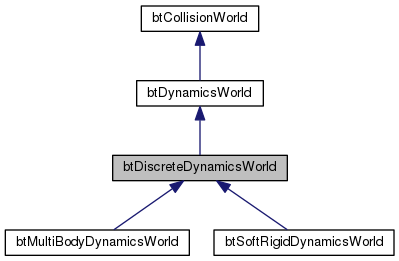
\includegraphics[scale=0.5]{img/RigidBodies/btDiscreteDynamicsWorldGraph.png}
\caption{Inheritance diagram of \texttt{btDiscreteDynamicsWorld}}
\label{fig: btDDWgraph}
\end{figure}

With that, we directly come to Bullet's rigid body class: \verb+btRigidBody+, see \autoref{fig: btRBgraph}. The library offers three kinds of rigid bodies types:
\begin{enumerate}
\item \textbf{Dynamic rigid bodies}, with positive mass. Motion is controlled by rigid body dynamics.
\item \textbf{Fixed objects} with zero mass. They are not moving (basically collision objects).
\item \textbf{Kinematic objects}, which are objects without mass, but the user can move them.
\end{enumerate}
We used objects of type 1. and 2., which we controlled by assigning them the corresponding mass. Hence, we could build dynamic (floating obstacles) and static objects (walls, boundaries) in our simulation. Furthermore, the \texttt{btRigidBody} class offers methods to access the properties of the objects such as 
\begin{itemize}
\item \texttt{getTotalForce():} Returning the force applied on the object
\item \texttt{getLinearVelocity():} Returning the linear velocity
\item \texttt{getCenterOfMass():} Returning the current center of mass
\end{itemize}
to name a few. 

\begin{figure}
\centering
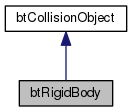
\includegraphics[scale=0.5]{img/RigidBodies/btRigidBodyGraph.png}
\caption{Inheritance diagram of \texttt{btRigidBody}}
\label{fig: btRBgraph}
\end{figure}

Finally, Bullet also offers the possibility to assign a shape to a \texttt{btRigidBody} object. Here, a shape object can be rather seen as a pattern than an actual object, since multiple rigid bodies can share the same shape object. The class in Bullet is called \texttt{btCollisionShape}. See \autoref{fig: btCSgraph} in the appendix, for an inheritance diagram which shows the amount of different shapes this family of classes provides. From convex shapes over concave shapes to compound shapes which one can freely design. The two shapes that we use are \texttt{btCylinderShape} and \texttt{btBoxShape}, see \autoref{fig: btCylSgraph} and \autoref{fig: btBoxSgraph}. By assigning a height of 1 to the cylinder we received a circle shape; the box shape was used for rectangles and squares. The idea was to later move on to more complex polygons, of course.
\begin{figure}[ht]
\centering
\begin{minipage}{.45\linewidth}
\centering
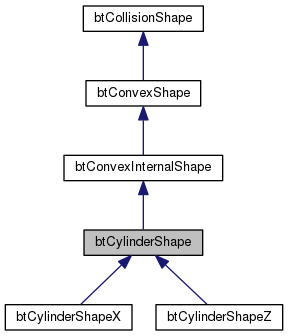
\includegraphics[scale=0.5]{img/RigidBodies/btCylinderShapeGraph.png}
\caption{Inheritance diagram of \texttt{btCylinderShape}}
\label{fig: btCylSgraph}
\end{minipage}
\hspace{.05\linewidth}
\begin{minipage}{.45\linewidth}
\centering
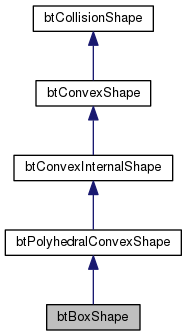
\includegraphics[scale=0.5]{img/RigidBodies/btBoxShapeGraph.png}
\caption{Inheritance diagram of \texttt{btBoxShapeGraph}}
\label{fig: btBoxSgraph}
\end{minipage}
\end{figure}

\subsubsection{Implementation}
In this section we want to take a look at our actual implementation. For that, the general structure is depicted with the help of an UML diagram, see \autoref{fig: RBUMLgraph}. Although the diagram shows a few of the most important methods, its focus lies more on the connection between the classes and the general structure. In the following, we want to give a simple introduction to the individual classes. All of them are also documented with the help of \emph{Doxygen} \cite{Doxygen}. Hence, to get more detailed information about the properties, members and methods of each class, create the Doxygen documentation by calling \texttt{doxygen Doxyfile} in the topmost folder of the source code. The main page of the documentation can then be found in \texttt{/html/index.html}.
\begin{figure}[ht]
\centering
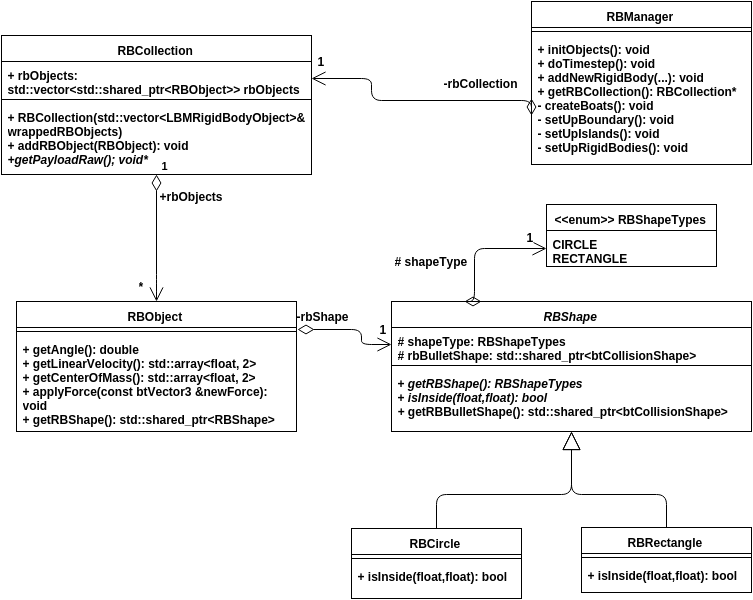
\includegraphics[scale=0.42]{img/RigidBodies/RigidBodyUML.png}
\caption{UML diagram of rigid body classes}
\label{fig: RBUMLgraph}
\end{figure}

\subsubsection*{RBObject and RBShape}
To wrap Bullet, we developed our own classes which we named \texttt{RBObject} and \texttt{RBShape}, which wrap \texttt{btRigidBody} and \texttt{btCollisionShape} respectively. The two specific shapes, we implemented by now are \texttt{RBCircle} and \texttt{RBRectangle}, see \autoref{fig: RBShape} for the specific inheritance diagram. \todointern{Benni}{should this be moved to the respective interfaces?}
\texttt{RBObject} on the other hand includes all the methods from Bullet which we need to transfer information for the LBM simulation and the visualization, like \texttt{getLinearVelocity()} and \texttt{getCenterOfMass()} as mentioned above. 
\begin{figure}[ht]
\centering
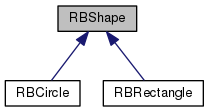
\includegraphics[scale=0.5]{img/RigidBodies/RBShapeGraph.png}
\caption{Inheritance diagram of \texttt{RBShape}}
\label{fig: RBShape}
\end{figure}

\subsubsection*{RBCollection}
We furthermore wrote a class \texttt{RBCollection} which is a container class for all generated \texttt{RBObjects}. \texttt{RBCollection} is also responsible for the communication to LBM and visualization, since it is a derived class from \texttt{CPipelinePacket}. With methods like \texttt{getLBMOBjectWrapperBegin()} or \texttt{getPayloadRaw()} it gives access to different pieces of information transferred between the stages. 

\subsubsection*{RBManager}
\label{sec: rbManager}
The class \texttt{RBManager} has a \texttt{btDiscreteDynamicWorld} as member, control over the \texttt{RBCollection} and is hence responsible for the simulation. By calling the class method \texttt{doTimeStep()} one implicitly calls the method \texttt{stepSimulation()} of \texttt{btDiscreteDynamicWorld}. 
\todointern{Benni}{should this part be moved to the interfaces?} Furthermore, \texttt{RBManager} is responsible for setting up the correct world with the help of the methods by using its  interface to image recognition (see \autoref{sec: interfaceImageRecognition}:
\begin{itemize}
\item \texttt{addNewRigidBody():} Adds a new rigid body to \texttt{RBCollection} and \texttt{btDiscreteDynamicWorld}.
\item \texttt{setUpIslands():} Sets up the islands sent from image recognition.
\item \texttt{setUpBoundary():} Sets up the boundary sent from image recognition.
\item \texttt{setUpRigidBodies():} Sets up the floating objects in the domain sent from image recognition.
\item \texttt{createBoats():} Sets up the boats based on the position given by image recognition.
\end{itemize}

\subsubsection{Discussion}
\tododone[inline]{Benni}{responsible for \textbf{Discussion} on RB and Bullet: Erik, Friedrich, Benni}
\begin{itemize}
\item was a bit of an overkill: in the end we only used circles anyhow.
\item better way: 
\begin{itemize}
\item first simple mock up with basic, easy functionality implemented on our own: explicit euler, circles, no performance optimization...
\item then wrap physics engine as soon as interfaces are defined and running, whole change under the hood
\end{itemize}
\end{itemize}

\subsection{Interfaces}
\tododone[inline]{Benni}{responsible for subsection \textbf{Interfaces} of RB: Friedrich -- DONE}
As it turned out during the project, the most complex task was to get the interfaces between the groups running. Rigid bodies needed interaction with all of them:
\begin{itemize}
\item \textbf{Input devices:} Boat is a rigid body and forces are applied from input devices.
\item \textbf{Image recognition:} Sends the information on the terrain, which is then implemented as a set of rigid bodies.
\item \textbf{Visualization:} Creates the visual output of objects depending on their properties.
\item \textbf{LBM:} Simulates the fluid-structure interaction between flow and objects.
\end{itemize}
If one these interfaces is working, the whole project gets stuck. Hence, the correct implementation of the interfaces was a crucial task.
Additionally an important goal was to completely hide the complexity of the Bullet library from the other groups and just supply them with the -- for the respective task -- relevant information.

In the following sections, we want to explain the implementations of the different interfaces to the other groups in more detail.
%\begin{itemize}
%\item RB have many interfaces! Most complex to LBM, but also many more interfaces with different demands.
%\item discrete version(LBM, ImgRecognition) vs. continuous version(Visu, RB Internal) of RBs
%\end{itemize}
\subsubsection{to Input Devices}
\tododone[inline]{Benni}{responsible for interface from RB \textbf{to Input Devices}: Erik?}
\begin{itemize}
\item how to model rowing
\item apply forces to bodies depending on input
\item in the end more time for finetuning would have been good!
\end{itemize}

\subsubsection{to Image Recognition}
\label{sec: interfaceImageRecognition}
\tododone[inline]{}{responsible for interface from RB \textbf{to Image Recognition}: Friedrich -- \textbf{DONE}}
The interface to image recognition works with the help of the \texttt{ProcessingManager} class (as also already described in \autoref{sec: imageProcessing}) which we included as member in \texttt{RBManager}. This class contains all the information needed for us to set up the correct boat starting positions, boundaries and rigid and static bodies. The methods of \texttt{ProcessingManager} which we used were:
\begin{itemize}
\item \texttt{boatCenters():std::vector<cv::Vec2f>} Returns a 2D vector with the position of the boats.
\item \texttt{outerBorder():Polygon} Returns a \texttt{Polygon} which holds the structure of the outer border
\item \texttt{rigidBodies():std::vector<Polygon>} Returns all rigid bodies, stored as \texttt{Polygon} objects.
\item \texttt{staticBodies():std::vector<Polygon>} Returns all static bodies, stored as \texttt{Polygon} objects.
\end{itemize} 
The corresponding private methods which call them were already described in \autoref{sec: rbManager} and are used by the public methods
\begin{itemize}
\item \texttt{initObjects()}, which sets up the boundary and the islands and
\item \texttt{handlePlayerArray()}, which initializes the rigid bodies and the boats
\end{itemize}
of \texttt{RBManager}. The interface is also visualised as an UML diagram in \autoref{fig: interfaceRBIR}.
\begin{figure}[ht]
\centering
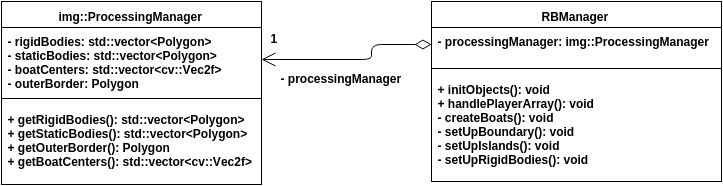
\includegraphics[scale=0.5]{img/RigidBodies/InterfaceRBImageRecogniton.png}
\caption{Interface between rigid bodies and image recognition.}
\label{fig: interfaceRBIR}
\end{figure}


For each \texttt{Polygon} given from the \texttt{ProcessingManager}, we can now calculate a center of mass. For rigid bodies (static or dynamic) we calculated the mean position of the polygon points as center of mass $\overrightarrow{x}$ and also the mean deviation $\hat{r}$ to approximate a radius $r$. By connecting the polygon points one after another with the help of rectangular shaped rigid bodies, we set up the boundary. The mass and shape is assigned depending on the type of the body and its volume (mass=0: static body, mass$>$0: dynamic body). We end up with four different kinds of rigid bodies which we approximated.
\begin{itemize}
\item \textbf{Boats:} RBCircle with position $\overrightarrow{x}$, radius $r=20$, mass$=0.6e4$ and moment of inertia$=1.2e7$.
\item \textbf{Islands:} RBCircle with position $\overrightarrow{x}$, radius $r=\hat{r}$, mass$=0$ and moment of inertia$=0$.
\item \textbf{Floating Objects:} RBCircle with position $\overrightarrow{x}$, radius $r=\hat{r}$, mass$=r^2$, and moment of inertia $=0$.
\item \textbf{Boundary:} RBRectangles connecting points of polygon, mass$=0$ and moment of inertia $=0$.
\end{itemize}
In the end, these new objects are added to the \texttt{btDiscreteDynamicWorld} and to \texttt{RBCollection}.


As one can easily imagine there is a lot of freedom in the exact parameter choice; the values taken here were derived from playing the game and getting a user feedback.
%\begin{itemize}
%\item how to model boundaries
%\item how to create different rigid bodies
%\end{itemize}

\subsubsection{to Visualization}
\tododone[inline]{Benni}{responsible for interface from RB \textbf{to Visualization}: Benni \textbf{DONE}}

For finally visualizing the rigid bodies we have to give access to the shape and the position of the rigid body. Our class \texttt{RBObject} already holds all this information. Therefore it was sufficient to grant -- through the \texttt{RBCollection} -- access to the \texttt{RBObject} objects:
\begin{itemize}
\item \texttt{getCenterOfMass()} and \texttt{getAngle()} give access to the position of the rigid body.
\item \texttt{getRBShape()} returns the \texttt{RBShape} of the body, which is either a \texttt{RBCircle} with its radius or a \texttt{RBRectangle} with the length of its two sides.
\end{itemize}
Representing shapes in an abstract way through the \texttt{RBShape} interface enabled us to completely hide Bullet from the visualization part of the pipeline while representing rigid body shapes in a proper and extensible way\footnote{Polygons could be easily added to our design, by simply adding a child class \texttt{RBPolygon} to the \texttt{RBShape} interface.}. 
\subsubsection{to LBM}
\tododone[inline]{Benni}{responsible for interface from RB \textbf{to LBM}: Erik?}
\begin{itemize}
\item how to send important quantities (discretization of continuous RB into cells, velocity of RB...)
\item how to receive important quantities (forces and torques from the fluid on the body)
\end{itemize}

\section{Visualization}
\tododone[inline]{Benni}{responsible for section \textbf{Visualization}: Benni?}

No funny stuff in here, only nice pictures

\section{Appendix}

\subsection{Rigid Bodies}
Inheritance diagram for \texttt{btCollisionShape} \autoref{fig: btCSgraph}.
\begin{figure}[ht]
\centering
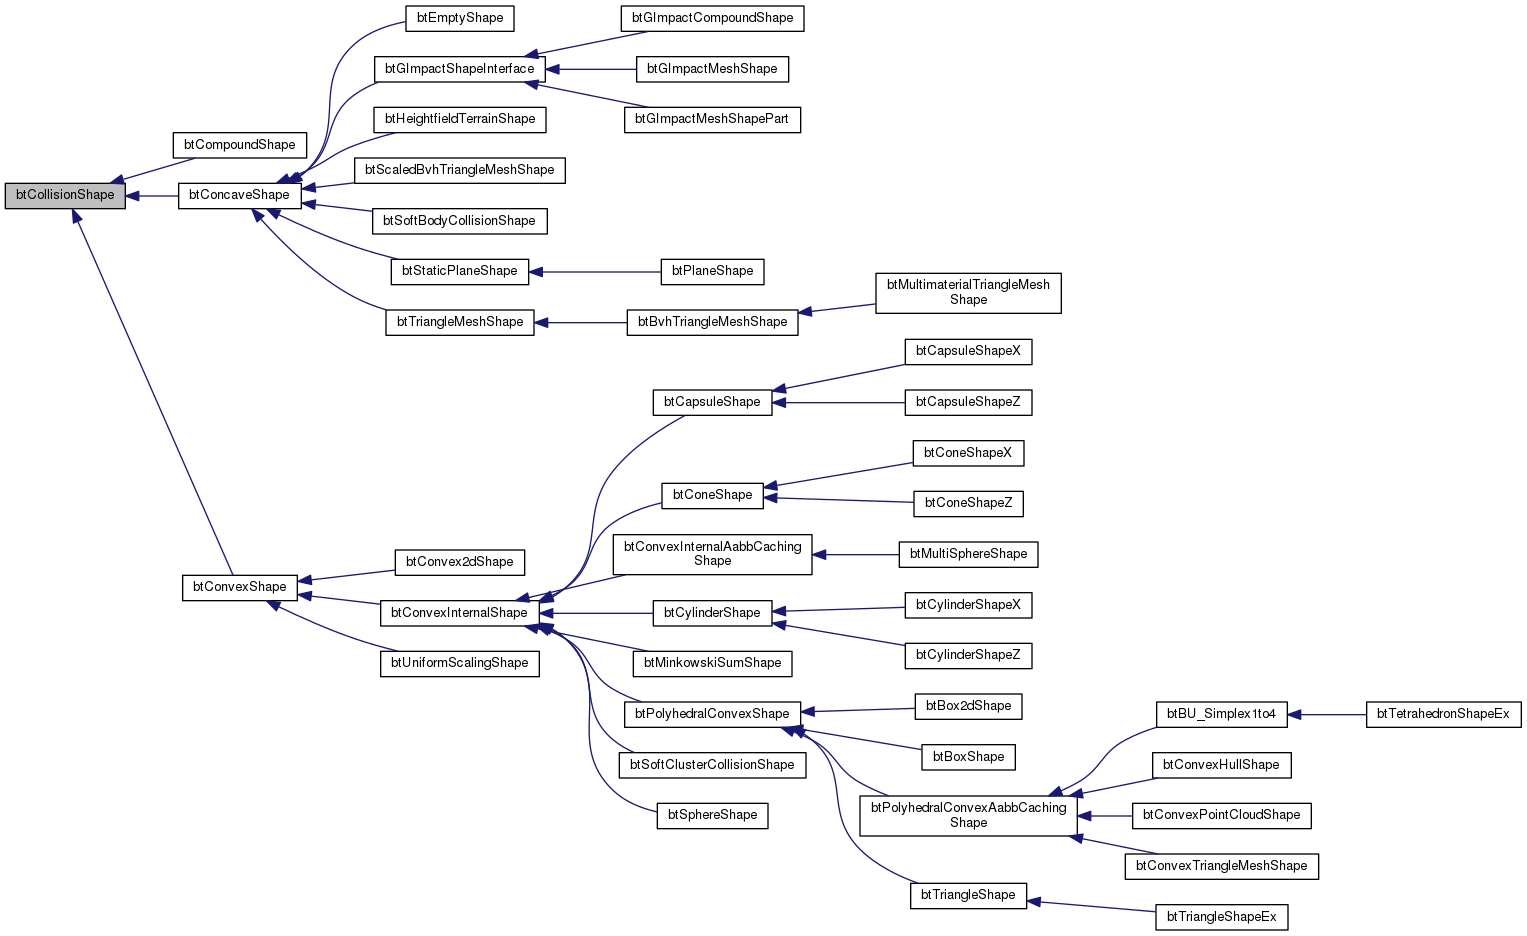
\includegraphics[scale=0.2]{img/RigidBodies/btCollisionShapeGraph.png}
\caption{Inheritance diagram of \texttt{btCollisionShape}}
\label{fig: btCSgraph}
\end{figure}

\clearpage
\newpage
\bibliographystyle{siam}
\bibliography{Sections/Bibliography/literature}

\end{document}
